\section{Project Outline}


\begin{comment}
    ever rising threat blah blah blah, hence why it is important to have good models for weather blah blah blah
\end{comment}



Classical weather forecasting methods generally consist of numerical weather prediction (NWP). This is the way in which computer simulations, in conjunction with sophisticated mathematical and physical models use the oceans and atmosphere to predict future weather conditions. These models do, however, come with an ever increasing complexity. Even with the most powerful supercomputers, "forecast skill" drops off after just the 6th day. These models are also fundamentally flawed by their intrinsic sensitivity and underlying chaotic nature further reducing efficacy as they produce further in time forecasts.

One way to overcome this is to take a data driven approach using machine learning techniques. This strategy is in its infancy when it comes to weather forecasting. Large meteorological entities such as the Met Office are, however, exploring methods such as pure Gaussian Process regression or a hybrid of both GP and NWP. These methods generally forecast for each city or region, assuming independence between each city. Although this is done with some success, particularly exceeding in the long term (6days \text{+}) forecasts, it could be argued that we are losing accuracy from that assumption. Weather features between cities are most likely correlated in some way. Hence I aim to explore the idea of taking a Bayesian Spatio-Temporal approach to weather forecasting, utilising both trends in time-series data of different weather features and also correlation in space between different locations of the United Kingdom. The ultimate goal is to produce a model that predicts precipitation in a given city using historical data from a variety of cities possibly as in Figure 1.

\begin{figure}[h]
      \centering
      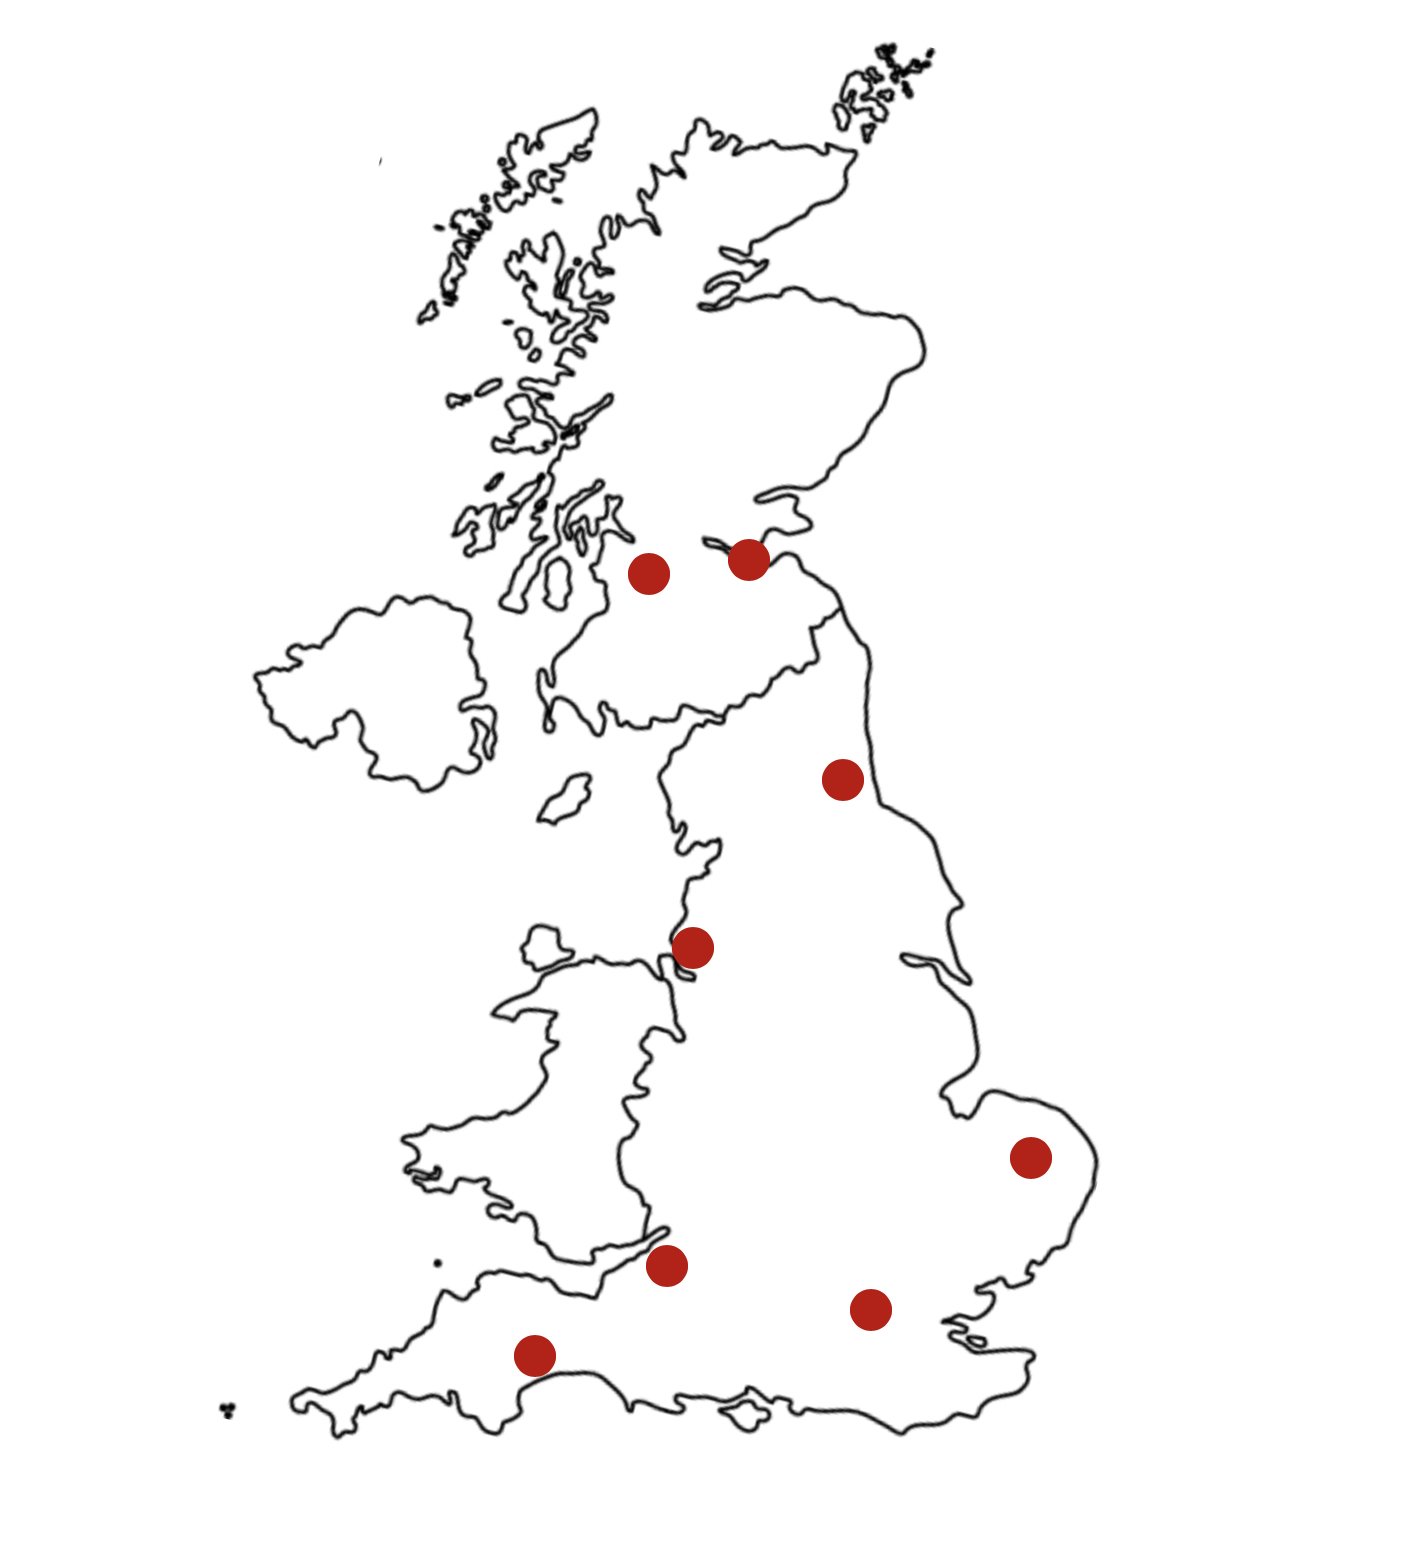
\includegraphics[width = 0.36\textwidth]{images/ukMap.png}
      
      \label{fig:ukMap}
  \end{figure}
  
\begin{itemize}
    

\item Edinburgh(55.953251, -3.188267) DONE
\item Glasgow(55.864239, -4.251806) DONE
\item Newcastle(54.978252 , -1.617780) DONE
\item Liverpool(53.408371,-2.991573) DONE 
\item Norwich(52.628101, 1.299350) DONE
\item Bristol(51.454514, -2.587910) DONE
\item London (51.509865, -0.118092) DONE
\item Exeter(50.721802, -3.533620) DONE\\ 
taking their lat/long readings from LatLong.net
\end{itemize}
  
  

The data-set will be taken from the company "Dark Sky" using their own API. I will be sampling daily weather data for the past few years. Many different weather features are provided, so I will need to be careful to overcome the curse of dimentionality and reduce the number of features down to a useful amount. We also want to remove or "merge" the highly correlated features to improve the model.


    

Although Spatio-Temporal forecasting research is also still in its infancy with regards to weather forecasting; there has been some serious progress in the field in general. From 





My evaluation will be ... cross validation of some sort?
